\chapter{Introduction}

The world is moving into a digital era. Computers are becoming more and more
intertwined in our daily lives. Many people spend time on the Internet, not just
for fun or gathering information, but also for social interaction, shopping or
on-line banking. Not only do our activities take place in a digital world,
existing systems are also moving to digital alternatives. Paper train tickets
are being replaced by electronic public transport cards. Identity documents,
\index{identity!documents} such as passports and identity cards, are equipped
with electronic chips to hold digital copies of the identity data printed on the
document. Sometimes even additional information is stored in these chips, such
as fingerprints or other biometric data.

Unfortunately, most digital systems use a simple approach to identify entities, including users;
they just associate them with a unique identifier\index{unique identifier}.
While this is convenient for bookkeeping, it also has a big drawback with
respect to privacy. Using these unique identifiers\index{unique identifier}, it
is easy to trace the user. This was already the case for tracking 
activities on the Internet, but now real world actions can easily be
traced as well through the use of public transport cards or digital identity
documents.\index{identity!documents}

In a security context, these unique identifiers\index{unique identifier} are
used to identify entities during authentication\index{authentication} and/or
authorisation\index{authorisation} processes, but in many use cases
identification is not necessary during such a transaction. For instance, when
you want to buy liquor, a merchant only needs to verify that you are of a
certain age. The same holds when boarding a train; the public transport system
only needs to know whether or not you are allowed to do so, and there is no
direct need for the system to know exactly who you are.

A more privacy-friendly approach is possible by using only specific properties
of the user, or \emph{attributes}\index{attribute}, as an alternative to
identities. Instead of providing lots of identity\index{identity!information}
information to a service provider, the user can just provide the required
attributes, such that the service can be accessed without the user revealing his
identity. For example, when you want to buy a bottle of wine you just prove that
you are over~18 (or~21) years of age, which is sufficient to
authorise\index{authorisation} the transaction, without revealing who you are.
To be more precise, it does not matter who you are, where
you live, or even what your age actually is. You are allowed to buy the wine, as
long as you satisfy the property that you have reached a certain age. This
illustrates that it is often more important \emph{what} you are than \emph{who}
you are.

\section{Attributes and Credentials}

Within this thesis, an attribute\index{attribute} will be understood as a
property or statement\index{attribute!statement} concerning a person. Examples
of attributes are:
\begin{multicols}{2}
\begin{itemize}
  \item I am a \textsf{student} (or \textsf{senior citizen})
  \item I am \textsf{over~12} (or \textsf{18}, or \textsf{21}, or \textsf{65})
  \item I have a \textsf{second class train pass}
  \item My \textsf{gender} is \textsf{male / female}
  \item My \textsf{loyalty status} for company \dots\ is \textsf{bronze / silver / gold / \dots}
  \item My \textsf{name} is \dots
  \item My \textsf{date of birth} is \dots
  \item My \textsf{address} is \dots
  \item My \textsf{social security number} is \dots
  \item I own the \textsf{bank account} with number \dots
\end{itemize}
\end{multicols}

Note that some of these attributes, like your bank account or social security
number, can be used to uniquely identify you, while other attributes are not
uniquely identifying: they apply to other people as well.

Informally, a person's identity\index{identity} can be seen as the collection
of all attributes\index{attribute} that hold for this person. In practice, many
transactions can be based on a minimal set of attributes, namely exactly those
attributes which are relevant or required to carry out the transaction. For
example one can think of the following scenarios\index{scenarios}:
\begin{itemize}
  \item If you wish to get a cheaper meal, show the \textsf{student} attribute,
    and for cheaper public transport you show that you are a \textsf{senior
    citizen}.
  \item If you buy an item in an on-line shop you need to reveal your
    \textsf{bank account} and \textsf{address} attributes, and possibly also
    your \textsf{loyalty status} attribute.
  \item When you buy a certain type of game or video on-line, you need to
    prove that you possess the attribute \textsf{over~12}, or \textsf{over~18}.
\end{itemize}
Note that in the last scenario, instead of using an attribute with the
\textsf{over~12} or \textsf{over~18} statement,\index{attribute!statement}
\index{statement|see{attribute, statement}} this property can also be proved
based on the \textsf{date of birth} attribute. This is then called a
\emph{derived attribute}.\index{attribute!derived}
\index{derived attribute|see{attribute, derived}}

There are several cryptographic systems for dealing with identities
\index{identity} based on attributes\index{attribute}. Typically these systems
distinguish attributes and credentials. Informally, a credential
\index{credential} is a \emph{cryptographic container \index{cryptographic
container} of attributes}. As a first approximation, one can think of a
credential as depicted in Figure~\ref{fig:Credential}. Examples of credentials
are~\cite{AlparJacobs2013}:
\begin{itemize}
  \item An \textbf{address} credential, containing for example the 
    \textsf{street}, \textsf{zipcode}, \textsf{city} and \textsf{country} 
    attributes.
  \item A (citizen) \textbf{identity} credential, containing for example the 
    \textsf{name}, \textsf{gender}, \textbf{date of birth}, and \textsf{social
    security number} attributes.
  \item A \textbf{student} credential, containing for example the 
    \textsf{student number}, \textsf{field of study}, \textsf{enrolment year} 
    and \textsf{university/college} attributes.
  \item A \textbf{festival} credential, containing for example the \textsf{festival name} and \textsf{date/time} attributes.
\end{itemize}

\begin{figure}[ht]
  \centering
  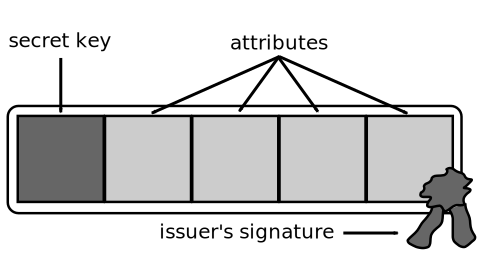
\includegraphics[scale=.5]{images/credential}
  \caption{A visual representation of an attribute-based credential.}
  \label{fig:Credential}
\end{figure}

\subsection{Credential Issuance and Verification}

Credentials are \emph{issued} and \emph{verified}, whereas attributes can be
\emph{disclosed} or \emph{proved} during verification. A credential is issued
by an authority, the \emph{issuer}\index{issuer}, which can assess that the
attribute statements\index{attribute!statement} in the credential hold for the
individual they are issued to. This individual, the \emph{user}, can
subsequently use this credential to \emph{prove} to another party, the
\emph{verifier}\index{verifier}, that she has a certain qualification,
competence, or property.

An issuer and a user together construct a new credential using the issuance
procedure\index{issuance procedure}. First the user authenticates
\index{authentication} to the issuer in some reliable but (for this
description) unspecified manner (which may be face-to-face). Once the
authentication\index{authentication} succeeds, the issuer collects the
attributes\index{attribute} for this user from its trusted sources. The user
and issuer then carry out a cryptographic protocol in which the attributes
are combined into a credential signed by the issuer. The resulting credential
contains the attributes concerning the user and also the user's personal key (as
depicted in Figure~\ref{fig:Credential}).

The fact that the attributes\index{attribute} hold for the owner of a
credential is guaranteed both by the issuer's signature and by the embedded
personal key of the owner. The secret key embedded in the credential plays an 
essential role in the verification procedure\index{verification procedure} of 
the credential, since it is supposed to be only known by the credential owner. 
Therefore this secret key, if properly protected, ensures that a credential 
cannot be transferred from one user to another.

\subsection{Selective Disclosure of Attributes}

A user may have several credentials, each containing some collection of
attributes\index{attribute}. When requesting a service from a service provider,
the user is required to authenticate\index{authentication} using one (or more)
of her credentials. In the verification process the user can choose to only
provide certain credentials; also, given a specific credential, the user may
choose to reveal only a selection\index{selection} of the attributes
\index{attribute} contained in the credential. By doing this, authentication
\index{authentication} becomes more privacy friendly. This verification process
is called \emph{selective disclosure}\index{selective disclosure}, involving
a verification protocol in which only a subset of the credential attributes
is revealed to the verifier while the other attributes are only proved to be
present in the credential. This allows a user to reveal only the necessary
attributes and prove that the credential belongs to her. The service provider
can verify all information that has been sent, including the issuer's signature.

The roles of a service provider and an issuer\index{issuer} can also be
combined: after verifying one credential, a new one can be issued. For instance,
after verifying an \textsf{over~18} attribute\index{attribute} from an identity
\index{identity} credential, a liquor shop might choose to issue a
\textsf{loyalty} credential.

In this thesis we stick to a simplistic approach to selective disclosure in
which an attribute index set\index{attribute!index set} $\A_D \subseteq \A$
determines which of the attributes\index{attribute} $\{a_i\}_{i \in \A}$
contained in the credential will be revealed to the verifier. Note that more
advanced proofs about attributes can be generated~\cite{IdemixCrypto2012}. For
example, the \textsf{over~18} statement \index{attribute!statement} derived
from \textsf{date of birth} attribute mentioned above, or that the current date
is within the validity period specified in a \textsf{train pass}
attribute~\cite{Rogaar2011}. This is, however, out of scope for this thesis.

\subsection{Security and Privacy}

The cryptographic nature of the credential-as-container concept includes the
following four security aspects.
\begin{itemize}
  \item The issuer's digital signature ensures \emph{authenticity}:
    \index{authenticity} the credential originates from the issuer, and this
    issuer\index{issuer} asserts that the attributes hold for the user.
  \item This signature also guarantees \emph{integrity}: \index{integrity} the
    attributes contained in the credential have not been altered since they were
    issued.
  \item A credential is \emph{non-transferable}\index{non-transferability} as
    it is bound to the secret key of the person involved in the issuance
    protocol. This secret key should be well protected, for instance via storage
    in the secure memory of a smart card\index{smart card} with a PIN.
  \item A credential \emph{hides}\index{hiding} its content, so it does not
    reveal the attributes it contains, unless these attributes are revealed
    during verification.
\end{itemize}
Furthermore, a credential can protect the privacy\index{privacy} of its owner
through the following two cryptographic properties.
\begin{itemize}
  \item \emph{Issuer unlinkability}\index{unlinkability!issuer}
    \index{issuer unlinkability|see{unlinkability!issuer}} ensures that any
    information that the issuer gathers during the issuing procedure cannot be 
    used to link a verification of the credential to its issuance.
  \item \emph{Multi-show unlinkability}\index{unlinkability!multi-show}
    \index{multi-show unlinkability|see{unlinkability, multi-show}} guarantees
    that when a credential is verified multiple times, these sessions cannot be
    linked.
\end{itemize}
The privacy of users is protected by these unlinkability properties even if the
credential issuer\index{issuer} and all verifiers collude. These properties can
be achieved in a variety of ways, as can be seen by the different
attribute-based credential technologies that have been proposed.

\section{Attribute-based Credential Technologies}

A number of technologies have been developed based on ideas described above, but
the main focus has been on the cryptography that enables such systems and less
on (efficient) implementations and their use cases. The implementations which
have been developed are mainly for ordinary computers, while our research
focuses on implementing such technologies on smart cards.\index{smart card} This approach offers
various new usage scenarios, like privacy-friendly public transport cards and
identity\index{identity!documents} documents, but also faces difficulties due
to the limited capabilities of smart card platforms and hardware (see
Section~\ref{sec:smartcards}).

The first attribute-based credentials have been described by
Chaum~\cite{Chaum1985} in 1984. In this section we introduce a number of recent
technologies which provide attribute-based credentials, which use various
cryptographic methods to achieve the security and privacy properties mentioned
above.

\subsection{Randomisable Certificates}

Credentials based on randomisable certificates\index{randomisable certificates},
such as Verheul's self-blindable credentials~\cite{Verheul01}, employ special
cryptographic techniques enabling the certificate structures to be randomised
using blinding factors while preserving their verifiability. The benefit of this
\index{signature randomisation} approach is that the use of such credentials is
untraceable. To achieve this, the users can blind their credentials before they
are verified, such that two occurrences of the same credential cannot be
recognised.

These credentials, as proposed by Verheul~\cite{Verheul01}, are discussed in
detail in Chapter~\ref{chp:self-blindable} as well as our efficient smart card
implementations~\cite{BatinaHJMV10,HoepmanJV10} using elliptic curve
cryptography.

\subsection{Single-show Credentials}

Another approach is to use single-show credentials\index{single-show
credentials} in combination with a blind signature protocol\index{blind
signature}. Here the issuance involves creating a blind signature which
conceals the resulting credential from the issuer. Therefore, the verification
instances of this credential cannot be related to the issuing phase. These
credentials are called single-show since they do not provide the multi-show
unlinkability property\footnote{Multi-show unlinkability for these schemes can
be realised by issuing multiple credentials for the same set of attributes which
can later be verified independently.} and can therefore be linked when they are
used multiple times. Hence these credentials serve as a pseudonym.
\index{pseudonym}

Examples of this approach are the credentials proposed by
Brands~\cite{Brands2000}, which are used in Microsoft's U-Prove
technology~\cite{U-Prove_Crypto2013}, and the light-weight credentials described
by Baldimtsi and Lysyanskaya~\cite{BaLy2012}.

A previous attempt to implement such technology on a smart card by Tews and
Jacobs~\cite{TewsJacobs09}, based on Brands' description~\cite{Brands2000},
resulted in a highly involved application with running times in the order of
5--10 seconds which make it not really usable in practice. Our smart card
implementation~\cite{MostowskiVullers11} of U-Prove not only has a much better
performance but is also, except for some minimal limitations, compatible with
the development kits provided by Microsoft. We discuss this implementation and
the U-Prove technology~\cite{U-Prove_Crypto2013} in detail in
Chapter~\ref{chp:uprove}.

\subsection{Multi-show Credentials}\index{multi-show credentials}

The use of zero-knowledge proofs\index{zero-knowledge proof} allows a user to
prove ownership of a credential without revealing the credential itself. This
achieves multi-show unlinkability, as the verifier does not see the credential.
Camenisch and Lysyanskaya~\cite{CamenischLysyanskaya2001,CamenischLysyanskaya2003}
combine such proofs with randomisation of the issuer's signature\index{signature
randomisation} to provide issuer unlinkability\index{unlinkability!issuer}.
Their credential scheme was used as the basis for IBM's Identity Mixer
\index{Identity Mixer} technology~\cite{IdemixCrypto2012} and the direct
anonymous attestation\index{direct anonymous attestation}
scheme~\cite{BrickellCC04} which has been adopted in the Trusted Platform Module
specification~\cite{TPM_1.2} as the method for remote authentication
\index{authentication!remote} of a hardware module.

In 2009 Bichsel et~al.~\cite{BichselCGS2009} implemented Identity Mixer
\index{Identity Mixer} on a Java Card\index{Java Card} whereas Sterckx et
al.~\cite{Sterckx09} did the same for direct anonymous attestation\index{direct
anonymous attestation}. They provide the first proper implementations of
attribute-based credentials on smart cards. The major drawback of these
implementations is the running time of several seconds which is still too much
for being really practical.

Our efficient implementation~\cite{VullersAlpar2013} of the Identity Mixer
\index{Identity Mixer} technology is described in Chapter~\ref{chp:idemix},
together with a detailed description of the underlying technology.

\subsection{Shared Keys\label{sec:nPA}}

The schemes that we have described so far are (to the best of our knowledge) the
only candidates that provide privacy by design and could be implemented on a
smart card. However, we should also briefly mention the approach used by
the German national identity card (nPA)\footnote{%
\url{http://www.personalausweisportal.de/}}, where a limited form of (anonymous)
\index{attribute!anonymous} attribute use is achieved by altering the existing
elliptic curve based electronic identity protocols by sharing private keys
\index{shared keys} across large batches\footnote{The size of these batches is in the order of a million cards per batch.} of cards~\cite{Kugler2010}. The
protocol itself provides restricted access to the card by means of the so-called
card verifiable certificate mechanism~\cite{EAC20} and allows for selective
disclosure of attributes, depending on the rights specified in the certificate
(for example, a liquor store is only authorised\index{authorisation} to check
for the \textsf{over~18} attribute). Signed attributes are partly anonymous
\index{attribute!anonymous} because of the sharing of the signing keys between
batches of cards, such that a signature cannot be linked to a single card.

\section{Smart Cards\label{sec:smartcards}}
\index{smart card|(}

During our research we try to assess how fast privacy-friendly protocols can be
executed when run on a modern smart card\index{smart card}. Hence
implementing our prototypes requires an open smart card platform\index{smart
card!platform} that also provides the necessary cryptographic hardware support,
as previous research~\cite{TewsJacobs09} clearly shows that, in terms of
performance, purely software-based prototypes\footnote{These prototypes are 
implemented without the use of dedicated cryptographic routines.} are not 
sufficient for realistic use. In practice that leaves us with two possible 
smart card platforms, Java Card\index{Java Card} and MULTOS\index{MULTOS}, 
described below.

Regardless of the software platform operating the card, all smart cards provide
the same external functionality. A smart card is an embedded device that
communicates with the environment through Application Protocol Data Units
(APDUs)\index{APDU}, byte arrays formatted according to the ISO7816-4
specification~\cite{ISO7816_4}. Most notably, the APDUs constrain the
communication payload to roughly 256 bytes in each direction for a single APDU
exchange. The permanent storage of the card (EEPROM memory\index{EEPROM}) is
considered highly secure, accessible only through the APDU commands offered by
the application, which in turn are subject to any authentication
\index{authentication} and secure messaging requirements that the card
application may impose.

\subsection{Java Card}\label{sec:javacard}\index{Java Card|(}

Java Card~\cite{Chen00} is a now well-established smart card platform based on
a tailored, cut-down version of the Java platform. One of the main features of
Java Card is software interoperability. This allows a developer to write a smart
card application, or applet\index{applet|see{Java Card, applet}}\index{Java
Card!applet}, in Java which can be executed on the Java Card virtual machine.
The Java Card\index{Java Card!API} API can then be used as an interface to the
(cryptographic) hardware of the smart card, making the applet (almost) fully
independent of the underlying hardware and operating system of the actual smart
card.

\subsubsection{Virtual Machine}

The Java Card virtual machine\index{virtual machine}
specification~\cite{jcvm222} defines a restricted subset of the Java programming
language, though it preserves many of the object-oriented features including
inheritance, interfaces, and exceptions. The specification also defines a
Java-compatible virtual machine for smart cards which consists of two parts; one
part external to the card and the other running on the card itself. The on-card
virtual machine interprets the bytecodes and manages the classes and objects.
The other part is a converter tool, that loads, verifies, and further prepares
the Java classes in a card applet for on-card execution.

\subsubsection{Memory Management}

On a Java Card device, memory is the most valuable resource\footnote{A typical 
modern smart card only has 36 to 144 KB of EEPROM for storing data and 4 to 8KB
of RAM (which is only partially available to an application developer) for
session data and computations.}. In most Java Card implementations a garbage
collector is not available. When an object is created, the object and its
contents are preserved in non-volatile 
memory\index{non-volatile memory} (EEPROM\index{EEPROM}), making it available 
across sessions. Access to the volatile memory\index{volatile memory} 
(RAM\index{RAM}) is provided through the Java Card API, which defines methods 
that allow you to create transient data storage at run-time.

In a Java Card environment a few rules should be taken into account to prevent
wasting memory at run-time. Arrays and primitive types should be allocated at
object creation time, and object creation should be minimised in favour of
object reuse. All arrays and objects that an applet needs during its lifetime 
should be created all in one go, when an applet is installed, such that no 
additional dynamic memory allocation is needed once the applet is up and 
running. To promote reuse, objects should remain in scope or referenced for the
life of the applet, and their state reset as appropriate before reuse.

\subsubsection{Application Programming Interface}

The Java Card API\index{Java Card!API} is carefully designed to support the
smart card environment and has several built-in security features. For example,
it provides predefined Java classes for hardware supported cryptographic key
storage (with possible internal encryption). To account for different hardware
profiles of a card, parts of the Java Card API implementation are made optional.
For example, our development cards based on NXP SmartMX chips support both RSA
\index{RSA cryptography} and elliptic curve cryptography\index{elliptic curve
cryptography} in hardware and expose this functionality through the API, while
other cards may only support RSA, in which case all method calls related to
elliptic curve cryptography result in a Java exception.

This brings us to the main shortcoming of the Java Card platform from our point
of view. The Java Card API is predefined and aimed at high-level functionality.
For example, for RSA based cryptography it is only possible to generate keys of
predefined RSA lengths (such as 512 and 1024 bits) and perform RSA operations
according to standard specifications, such as PKCS \#1~\cite{PKCS_1}. The
underlying mathematical operations, such as modular exponentiation, are not
available to a developer. Since all of the protocols that we are interested in
require access to such cryptographic operations (in large modulo prime and/or
elliptic curve domains), this is a practical show stopper. Similar problems have
been reported by others~\cite{BichselCGS2009,Sterckx09} regarding the implementation of
cryptographic protocols on a Java Card. Even more, an efficient implementation
of the e-passport standard~\cite{EAC20} on a Java Card also requires
cryptographic routines not anticipated by the standard Java Card API. In this
case, due to high demand, Java Card producers decided to enrich the Java Card
API with proprietary extensions to support e-passport standards~\cite{NXP09}.
But this only solves the problem for one application type and, moreover, makes
the platform non-interoperable.
\index{Java Card|)}

\subsection{MULTOS}\label{sec:multos}\index{MULTOS|(}

The goal of the MULTOS platform is to provide a secure hardware-independent
execution platform for smart cards. To this end, they developed a specification
for the execution and memory models, explained in more detail below, that all
MULTOS implementations must provide. Besides this mandatory part of the
specification there are also a number of optional elements, mostly concerning
cryptographic functionality that may or may not be available on a specific
hardware platform. An overview of which functionality is provided by which card
can be found in the MULTOS implementation reference~\cite{MIR2012}.

\subsubsection{Execution Model}

Applications on a MULTOS card are executed in a virtual machine\index{virtual
machine}, called the application abstract machine. The functionality of this
virtual machine is defined by the MULTOS specification to assure that
applications are portable, that is, independent of the actual chip
used\footnote{Application portability can be limited due to specific memory
requirements or dependencies on optional parts of the MULTOS specification.}.
The application abstract machine is a stack machine\index{stack machine} that
interprets instructions from the MULTOS executable language (MEL).

\subsubsection{Memory Model}

The virtual machine provides each application with its own memory space. Within
an application the code space, residing on non-volatile EEPROM\index{EEPROM}
\index{non-volatile memory|see{EEPROM}} storage, and data space, divided over
EEPROM (for persistent storage) and volatile RAM\index{RAM}\index{volatile
memory|see{RAM}}, are handled independently of each other. The memory of an
application is protected by a strong firewall. This means that applications
cannot access each others memory. The data of an application is divided over
three distinct memory areas, listed below.

\paragraph{Static memory} is the non-volatile storage for an application. It is
private to the application and cannot be accessed by the terminal or any other
application. MULTOS offers mechanisms to avoid corruption of the static memory
area such that this data remains consistent.

\paragraph{Public memory} is the volatile input/output buffer for an
application. Incoming command APDUs are held in public memory and outgoing
response APDUs are placed here. This buffer is also used to pass information
from one application to another when delegation is used. MULTOS guarantees that
data in this memory remains private to the running application until it exits
or delegates to another application. This means that it can be used as
temporary work space.

\paragraph{Dynamic memory} is the volatile storage for an application. It is
used to store session data, if any. The size of the session data area is fixed
when an application is loaded onto a card and it depends on the number of
variables declared. Furthermore, the dynamic memory contains the stack, which
is the application's work area. As mentioned before, the application abstract
machine operates as a stack machine, which means that this memory area is used
to perform many functions (and provide input for these functions). The size of 
the stack is limited by the size of the session data in the dynamic memory. 
Therefore, applications have to ensure that their dynamic memory use does not 
exceed the the limit of the used chip~\cite{MIR2012}. 

\subsubsection{Application Programming Interface}

Similar to the Java Card API\index{Java Card!API} routines, some of the
instructions are specified to be optional, mostly ones responsible for
cryptographic operations. A particular MULTOS card may or may not support the
optional instructions. For our implementation we used development cards based on
the SLE66 and SLE78 chips from Infineon. These particular
cards~\cite{MIR2012} support a wide range of modulo arithmetic
operations, a range which is sufficient to fully support all of the required
calculations. The more low-level and flexible MULTOS\index{MULTOS!API} API, as
opposed to the less flexible and more high level Java Card API, is the main 
reason to choose the MULTOS platform for the prototype implementations of the
cryptographic protocols discussed in this thesis.

For our prototypes we used the MULTOS C interface and bits of MEL assembly. For
simple smart card applications the C interface seems to provide an easier 
programming environment than Java, and allows for a more flexible (byte-level) 
memory management. Although C programming platforms are not type safe by 
definition (as opposed to Java), per application memory safety is guaranteed by
the MULTOS platform, regardless of the high-level language used during 
development.

\index{MULTOS|)}
\index{smart card|)}

\section{Contributions}

The goal of the research presented in this thesis has been to
\begin{center}\it
  develop efficient smart card implementations of attribute-based credentials
\end{center}
and
\begin{center}\it
  compare various cryptographic systems for attribute-based credentials.
\end{center}
This has resulted in a detailed description and discussion of the technologies
listed below, which can be found in Chapters~\ref{chp:self-blindable},
\ref{chp:uprove}, \ref{chp:idemix} and \ref{chp:discussion}. Additionally, a
large and essential part of this thesis consists of the efficient smart card
implementations for each of these technologies. The implementations themselves
will not be described in detail in this thesis; we refer the interested reader
to the source code repositories mentioned below. Instead, we concentrate on
performance results, and on general issues or problems that came up during the
implementation work.

The implementations developed during this research are available as open source
software, under the GNU General Public
License\footnote{\url{https://www.gnu.org/copyleft/gpl.html}}, version~3,
unless stated otherwise in the \texttt{LICENSE} file included in the root of
each repository. The source code of these implementations can be found in their
respective repositories, as specified below, at \url{https://github.com/pimvullers/}.

\subsubsection{Self-blindable Credentials}

The third chapter is based on two papers, \emph{Developing Efficient Blinded
Attribute Certificates on Smart Cards via Pairings}~\cite{BatinaHJMV10} which
is joint work with Lejla Batina, Jaap-Henk Hoepman, Bart Jacobs and Wojciech
Mostowski, and \emph{Privacy and Security Issues in e-Ticketing -- Optimisation
of Smart Card-based Attribute-proving}~\cite{HoepmanJV10} which is joint work
with Jaap-Henk Hoepman and Bart Jacobs. I presented this work at the 9th IFIP WG
8.8/11.2 International Conference on Smart Card Research and Advanced
Applications (CARDIS 2010).

\paragraph{Contribution}

My contribution in this chapter is the development and analysis of the
\emph{first} efficient smart card implementation of the self-blindable
credentials technology as well as the implementation of the corresponding host
software. This consists of:
\begin{itemize}
  \item the Java Card applet\index{Java Card!applet} (\texttt{sbcred\_javacard} repository\footnote{%
    \url{https://github.com/pimvullers/sbcred_javacard/}}),
    which provides the cryptographic operations on the smart card;
  \item the terminal\index{terminal} software (\texttt{sbcred\_terminal} repository\footnote{%
    \url{https://github.com/pimvullers/sbcred_terminal/}}),
    which provides the cryptographic operations for the issuer and verifier as
    well as the protocol interaction with the smart card; and
  \item an extension, (\texttt{bouncycastle-ext} repository\footnote{%
    \url{https://github.com/pimvullers/bouncycastle-ext/}}),
    to the Bouncy Castle cryptographic library\footnote{%
    \url{http://bouncycastle.org/java.html}}, which adds support for elliptic
    curve bilinear pairings.
\end{itemize}

\subsubsection{U-Prove}

The fourth chapter is based on the paper \emph{Efficient U-Prove Implementation
for Anonymous Credentials on Smart Cards}~\cite{MostowskiVullers11} which is
joint work with Wojciech Mostowski. I presented this work at the 7th
International ICST Conference on Security and Privacy in Communication Networks
(SecureComm 2011).

\paragraph{Contribution}

My contribution in this chapter is the analysis of the efficient smart card
implementation of the U-Prove technology as well as the development of the
terminal\index{terminal} software (\texttt{uprove\_terminal} repository\footnote{%
\url{https://github.com/pimvullers/uprove_terminal/}}), which builds upon the
U-Prove SDK\footnote{\url{http://archive.msdn.microsoft.com/uprovesdkjava/}}
and takes care of the protocol interaction with the smart card. Furthermore I
provided the pseudo code that allowed my co-author to develop the MULTOS
application\index{MULTOS!application} (\texttt{uprove\_multos} repository\footnote{%
\url{https://github.com/pimvullers/uprove_multos/}}), which provides the
cryptographic operations on the smart card.

\subsubsection{Identity Mixer}\index{Identity Mixer}

The fifth chapter is based on the paper \emph{Efficient Selective Disclosure on
Smart Cards using Idemix}~\cite{VullersAlpar2013} which is joint work with
Gergely Alp\'ar. I presented this work at the 3rd IFIP WG 11.6 Working
Conference on Policies and Research in Identity Management (IDMAN 2013).

\paragraph{Contribution}

My contribution in this chapter is the development and analysis of the efficient
smart card implementation of the Identity Mixer\index{Identity Mixer} technology, 
which is the first smart card implementation to include \emph{selective 
disclosure} of the attributes, as well as the implementation of the corresponding 
host software. This consists of:
\begin{itemize}
  \item the MULTOS application\index{MULTOS!application}\footnote{This has evolved into the IRMA
    application (\url{https://github.com/pimvullers/irma_card/}) which provides
    additional functionality, like secure messaging and an interface which
    allows the user to manage the credentials stored on the card.}
    (\texttt{idemix\_multos} repository\footnote{%
    \url{https://github.com/pimvullers/idemix_multos/}}), which provides the
    cryptographic operations on the card; and
  \item the terminal\index{terminal} software (\texttt{idemix\_terminal} repository\footnote{%
    \url{https://github.com/pimvullers/idemix_terminal/}}), which provides the
    protocol interaction between the smart card and our patched version of the
    Identity Mixer\index{Identity Mixer!cryptographic library} cryptographic
    library\footnote{\url{https://prime.inf.tu-dresden.de/idemix/}}
    (\texttt{idemix\_library} repository\footnote{%
    \url{https://github.com/pimvullers/idemix_library/}}).
\end{itemize}

This implementation is the most complicated and challenging one in this thesis.
Because of the complicated nature of the Identity Mixer\index{Identity Mixer} operations it was, at
first, not expected that a fast implementation could be realised on a smart
card. The successful development of this implementation laid the foundation for
the IRMA project\index{IRMA project}. This is an on-going research and development project focusing
on attribute-based credentials and their use in practice.

This thesis does not described the IRMA project in great detail but concentrates
on the smart card implementations of the underlying attribute-based credential
technologies. For more information concerning the IRMA project, please visit
\url{https://www.irmacard.org/}.
